\documentclass[12pt]{article}
\usepackage[utf8]{inputenc}
\usepackage[T1]{fontenc} % uses T1 fonts (better quality)
\usepackage{lmodern}
\usepackage[dvipsnames]{xcolor}
\usepackage[margin=1in]{geometry}
\usepackage{graphicx} \graphicspath{ {./Images/} }
\usepackage{pdfpages}
\usepackage{booktabs}   % for table borders
\usepackage{amsmath,bm}
\usepackage[makeroom]{cancel}
\usepackage{tikz} \usetikzlibrary{shapes,arrows}
\usepackage{minted} \usemintedstyle{friendly}
\usepackage{enumitem}
\begin{document}
 	\begin{center}
    \line(1,0){300}\\[0.25cm]
 	\Large{\bfseries ECE540: Homework \#2}\\
 	\textsc{\large David Kirby}\\
 	\textsc{\large Due: 24 September 2020}\\
 	\line(1,0){300}\\[0.75cm]
 	\end{center}

% Define block styles
% \tikzstyle{decision} = [diamond, draw, fill=blue!20,
%     text width=4.5em, text badly centered, node distance=3cm, inner sep=0pt]
% \tikzstyle{block} = [rectangle, draw,
%     text width=20em, text centered, rounded corners, minimum height=1em]
% \tikzstyle{line} = [draw, -latex']
% \tikzstyle{cloud} = [draw, ellipse,fill=red!20, node distance=3cm,
%     minimum height=2em]

\section*{Chapter 6}
\subsection*{Review Questions}
\begin{enumerate}
\item R3. What are some of the possible services that a link-layer protocol can offer to the network layer? Which of these link-layer services have corresponding services in IP\@? In TCP\@?
    \begin{itemize}
        \item Framing (IP \& TCP)
        \item Link access
        \item Reliable delivery (TCP)
        \item Error detection \& correction (IP \& TCP)
    \end{itemize}
\item R6. In CSMA/CD, after the fifth collision, what is the probability that a node chooses \(K = 4\)? The result \(K = 4\) corresponds to a delay of how many seconds on a 10 Mbps Ethernet?\\[1em]
        After the fifth collision, the probability that a node chooses \(K=4 \Rightarrow\frac{1}{2^5}=\frac{1}{32}\). At 10 Mbps, this equates to \(K\cdot512\cdot10^{-6}=204.8\rm{\mu s}\)
\item R9. How big is the MAC address space? The IPv4 address space? The IPv6 address space?
    \begin{itemize}
        \item MAC addresses: \(2^{48}\)
        \item IPv4 addresses: \(2^{32}\)
        \item IPv6 addresses: \(2^{128}\)
    \end{itemize}
\item R11. Why is an ARP query sent within a broadcast frame? Why is an ARP response sent within a frame with a specific destination MAC address?\\[1em]
Address Resolution Protocol resolves an IP address to a MAC address. If the IP address is unknown, i.e.\ it is not in the ARP module, a query is sent over broadcast frames to all the other hosts and routers on the subnet to determine the MAC address of the unknown IP address. Once a match has been found, the ARP response needs only to return this MAC address resolution to the querying host.
\end{enumerate}
\subsection*{Problems}
\begin{enumerate}
    \item P8. In Section 6.3, we provided an outline of the derivation of the efficiency of slotted ALOHA.\ In this problem we’ll complete the derivation.
    \begin{enumerate}
        \item Recall that when there are \textit{N} active nodes, the efficiency of slotted ALOHA is \(Np{(1 - p)}^{N-1}\). Find the value of \textit{p} that maximizes this expression.
        \begin{align*}
            \text{eff}&=Np{(1 - p)}^{N-1}
        \end{align*}
        To maximize, take derivative w.r.t. \(p\) and nullify:
        \begin{align*}
            \frac{\partial}{\partial p}(\text{eff})&=N{(1-p)}^{N-1}-Np(N-1){(1-p)}^{N-2}\\
            &=N\left((1-p)-p(N-1)\right){(1-p)}^{N-2}=0\\
            p^*&=\frac{1}{N}
        \end{align*}
        \item Using the value of \textit{p} found in (a), find the efficiency of slotted ALOHA by letting \textit{N} approach infinity. \textit{Hint}: \({(1 - 1/N)}^N\) approaches \(1/e\) as \textit{N} approaches infinity.
        \begin{align*}
            p^*&=\frac{1}{N}
        \end{align*}
        Plugging in \(p^*\) for \(p\) in the efficiency equation:
        \begin{align*}
            \text{eff}&=Np^*{(1 - p^*)}^{N-1}\\
            &=\cancelto{1}{N\frac{1}{N}}{(1-\frac{1}{N})}^{N-1}\\
            &=\frac{{(1-\frac{1}{N})}^{N}}{1-\frac{1}{N}}\\
            \lim_{N \to \infty}&=\frac{1}{e}
        \end{align*}
    \end{enumerate}
    \item P9. Show that the maximum efficiency of pure ALOHA is \(1/(2e)\). \textit{Note}: This problem is easy if you have completed the problem above!
    \begin{align*}
        \text{eff}&=Np{(1 - p)}^{2(N-1)}
    \end{align*}
    To maximize, take derivative w.r.t. \(p\) and nullify:
    \begin{align*}
        \frac{\partial}{\partial p}(\text{eff})&=N{(1-p)}^{2(N-2)}-2Np(N-1){(1-p)}^{2(N-3)}\\
        &=N\left((1-p)-2p(N-1)\right){(1-p)}^{2(N-3)}=0\\
        p^*&=\frac{1}{2N-1}
    \end{align*}

    \item P12. Graph the efficiency of slotted ALOHA and pure ALOHA as a function of \textit{p} for the following values of \textit{N}:
    \begin{enumerate}
        \item \(N=10\).
        \item \(N=30\).
        \item \(N=50\).
    \end{enumerate}
    \inputminted[frame=lines,linenos]{python}{./Matlab/ECE540_Ch6_P12_1.m}
    \begin{figure}[h!]
        \centering
        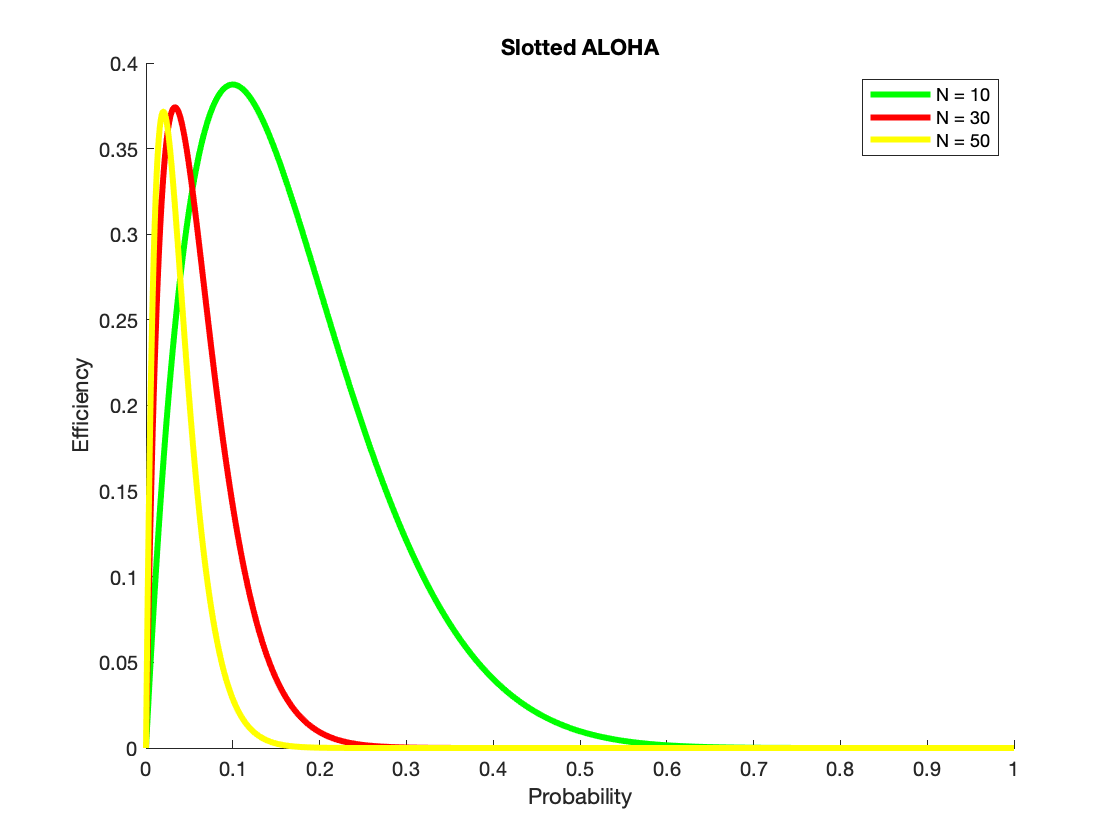
\includegraphics[width=0.85\textwidth]{./Matlab/fig1.png}
    \end{figure}
    \inputminted[frame=lines,linenos]{python}{./Matlab/ECE540_Ch6_P12_2.m}
    \begin{figure}[h!]
        \centering
        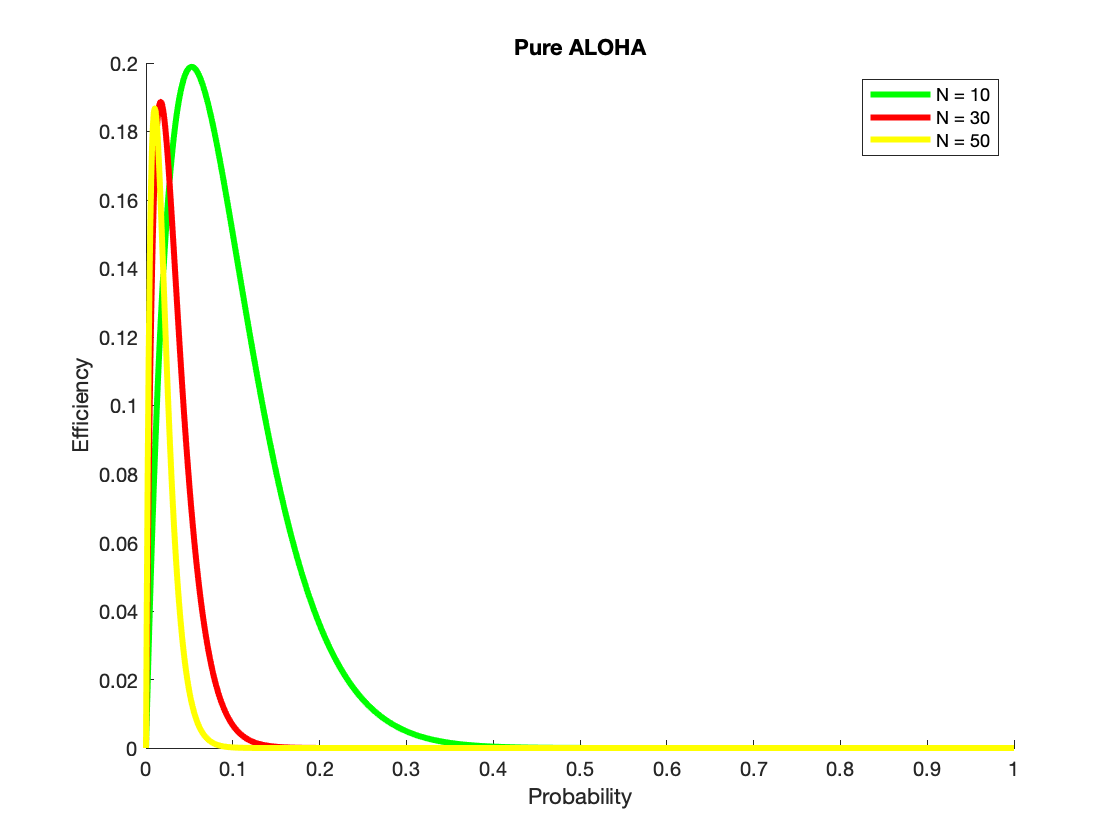
\includegraphics[width=0.85\textwidth]{./Matlab/fig2.png}
    \end{figure}
    \newpage
    \item P13. Consider a broadcast channel with \textit{N} nodes and a transmission rate of \text{R} bps. Suppose the broadcast channel uses polling (with an additional polling node) for multiple access. Suppose the amount of time from when a node completes transmission until the subsequent node is permitted to transmit (that is, the polling delay) is \(d_{\mathrm{poll}}\). Suppose that within a polling round, a given node is allowed to transmit at most \textit{Q} bits. What is the maximum throughput of the broadcast channel?
    \begin{align*}
        \text{Max bits per polling round}&=N\cdot Q\\
        \text{Rate to send max bits}&=\frac{N\cdot Q}{R}\\
        \text{Polling delay per polling round}&=N\cdot d_{\mathrm{poll}}\\
        \text{Duration of polling round}&=\frac{N\cdot Q}{R}+N\cdot d_{\mathrm{poll}}\\
        \text{Max throughput}&=\frac{NQ}{\frac{N\cdot Q}{R}+N\cdot d_{\mathrm{poll}}}\\
        &=\frac{R}{1+\frac{d_{\mathrm{poll}}\cdot R}{Q}}
    \end{align*}
    \item P14. Consider three LANs interconnected by two routers, as shown in Figure 6.33.
    \begin{figure}[h!]
        \centering
        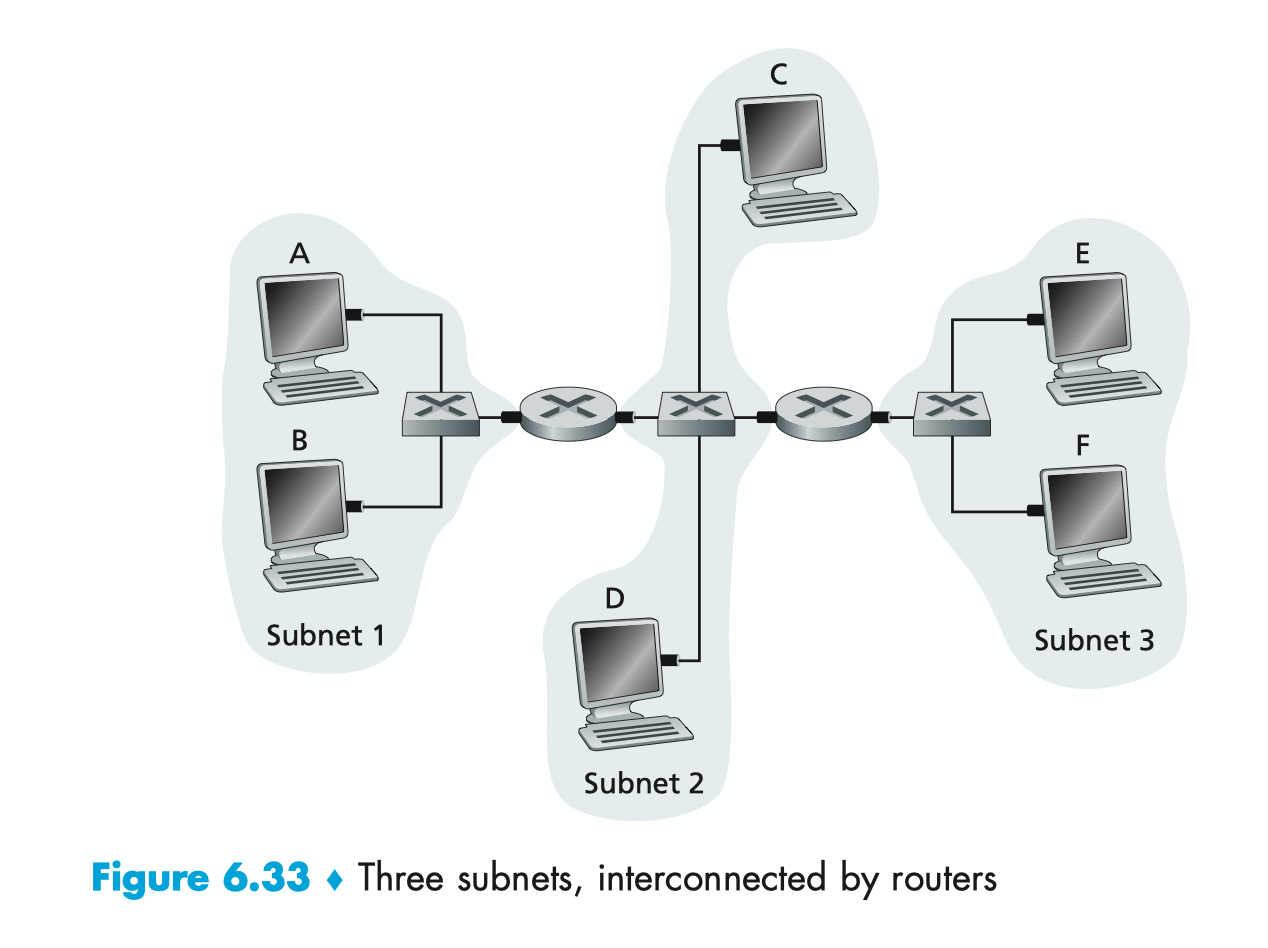
\includegraphics[width=0.95\textwidth]{Fig6.33.png}
    \end{figure}
    \newpage
    \begin{enumerate}
        \item Assign IP addresses to all of the interfaces. For Subnet 1 use addresses of the form 192.168.1.xxx; for Subnet 2 uses addresses of the form 192.168.2.xxx; and for Subnet 3 use addresses of the form 192.168.3.xxx.\\[1em]
        For (a) and (b), please see Figure 6.33 labeled above.
        \item Assign MAC addresses to all of the adapters.
        \item Consider sending an IP datagram from Host E to Host B. Suppose all of the ARP tables are up-to-date. Enumerate all the steps, as done for the single-router example in Section 6.4.1.
        \begin{enumerate}
            \item Request for router IP \texttt{192.168.3.002}.
            \item ARP table maps router IP \texttt{192.168.3.002} to MAC \texttt{88--88--88--88--88--88}.
            \item Forwarding tables determine datagram must be sent to next subnet router at \texttt{192.168.2.002}.
            \item Datagram is then sent through router \texttt{192.168.2.003} from MAC\\ \texttt{55--55--55--55--55--55} to MAC \texttt{44--44--44--44--44--44}.
            \item Router at \texttt{192.168.1.002} then receives and recognizes the destination IP address \texttt{192.168.1.003} at Host B with MAC \texttt{22--22--22--22--22--22}.
        \end{enumerate}
        \item Repeat (c), now assuming that the ARP table in the sending host is empty (and the other tables are up to date).
        \begin{enumerate}
            \item Request for router IP \texttt{192.168.3.002}.
            \item The sending Host (E), is now unaware of the IP of router \texttt{192.168.3.002}, so it must send out a query packet to the entire subnet using a broadcast Ethernet frame. Once the router at \texttt{192.168.3.002} receives the broadcast message, it sends a response packet using an Ethernet frame advertising its MAC address as \texttt{88--88--88--88--88--88}. The remaining steps are the same as in part (c).
            \item ARP table maps router IP \texttt{192.168.3.002} to MAC \texttt{88--88--88--88--88--88}.
            \item Forwarding tables determine datagram must be sent to next subnet router at \texttt{192.168.2.002}.
            \item Datagram is then sent through router \texttt{192.168.2.003} from MAC\\ \texttt{55--55--55--55--55--55} to MAC \texttt{44--44--44--44--44--44}.
            \item Router at \texttt{192.168.1.002} then receives and recognizes the destination IP address \texttt{192.168.1.003} at Host B with MAC \texttt{22--22--22--22--22--22}.
        \end{enumerate}
    \end{enumerate}
    \newpage
    \item P21. Consider Figure 6.33 in problem P14. Provide MAC addresses and IP addresses for the interfaces at Host A, both routers, and Host F. Suppose Host A sends a datagram to Host F. Give the source and destination MAC addresses in the frame encapsulating this IP datagram as the frame is transmitted \textit{(i)} from A to the left router, \textit{(ii)} from the left router to the right router, \textit{(iii)} from the right router to F. Also give the source and destination IP addresses in the IP datagram encapsulated within the frame at each of these points in time.\\[1em]
    Using the same MAC and IP numbering as shown in P14:
    \begin{enumerate}[label= (\roman{*})]
        \item MAC \& IP Addresses (respectively) from A to the left router
        \begin{align*}
            \text{Source:} &=\texttt{00--00--00--00--00--00}\quad \& \quad \texttt{192.168.1.001}\\
            \text{Destination:} &=\texttt{11--11--11--11--11--11}\quad \&\quad\texttt{192.168.3.003}
        \end{align*}
        \item from the left router to the right router
        \begin{align*}
            \text{Source:} &=\texttt{44--44--44--44--44--44}\quad \& \quad \texttt{192.168.1.001}\\
            \text{Destination:} &=\texttt{55--55--55--55--55--55}\quad \&\quad\texttt{192.168.3.003}
        \end{align*}
        \item from the right router to F
        \begin{align*}
            \text{Source:} &=\texttt{88--88--88--88--88--88}\quad \& \quad \texttt{192.168.1.001}\\
            \text{Destination:} &=\texttt{99--99--99--99--99--99}\quad \&\quad\texttt{192.168.3.003}
        \end{align*}
    \end{enumerate}
    \item P22. Suppose now that the leftmost router in Figure 6.33 is replaced by a switch. Hosts A, B, C, and D and the right router are all star-connected into this switch. Give the source and destination MAC addresses in the frame encapsulating this IP datagram as the frame is transmitted \textit{(i)} from A to the switch, \textit{(ii)} from the switch to the right router, \textit{(iii)} from the right router to F. Also give the source and destination IP addresses in the IP datagram encapsulated within the frame at each of these points in time.\\[1em]
    Using the same MAC and IP numbering as shown in P14:
    \begin{enumerate}[label= (\roman{*})]
        \item MAC \& IP Addresses (respectively) from A to the switch
        \begin{align*}
            \text{Source:} &=\texttt{00--00--00--00--00--00}\quad \& \quad \texttt{192.168.1.001}\\
            \text{Destination:} &=\texttt{55--55--55--55--55--55}\quad \&\quad\texttt{192.168.3.003}
        \end{align*}
        \item from the switch to the right router
        \begin{align*}
            \text{Source:} &=\texttt{00--00--00--00--00--00}\quad \& \quad \texttt{192.168.1.001}\\
            \text{Destination:} &=\texttt{55--55--55--55--55--55}\quad \&\quad\texttt{192.168.3.003}
        \end{align*}
        \item from the right router to F
        \begin{align*}
            \text{Source:} &=\texttt{88--88--88--88--88--88}\quad \& \quad \texttt{192.168.1.001}\\
            \text{Destination:} &=\texttt{99--99--99--99--99--99}\quad \&\quad\texttt{192.168.3.003}
        \end{align*}
    \end{enumerate}
    \item P29. Consider the MPLS network shown in Figure 6.29, and suppose that routers R5 and R6 are now MPLS enabled. Suppose that we want to perform traffic engineering so that packets from R6 destined for A are switched to A via R6-R4-R3-R1, and packets from R5 destined for A are switched via R5-R4-R2-R1. Show the MPLS tables in R5 and R6, as well as the modified table in R4, that would make this possible.
    \begin{figure}[h!]
        \centering
        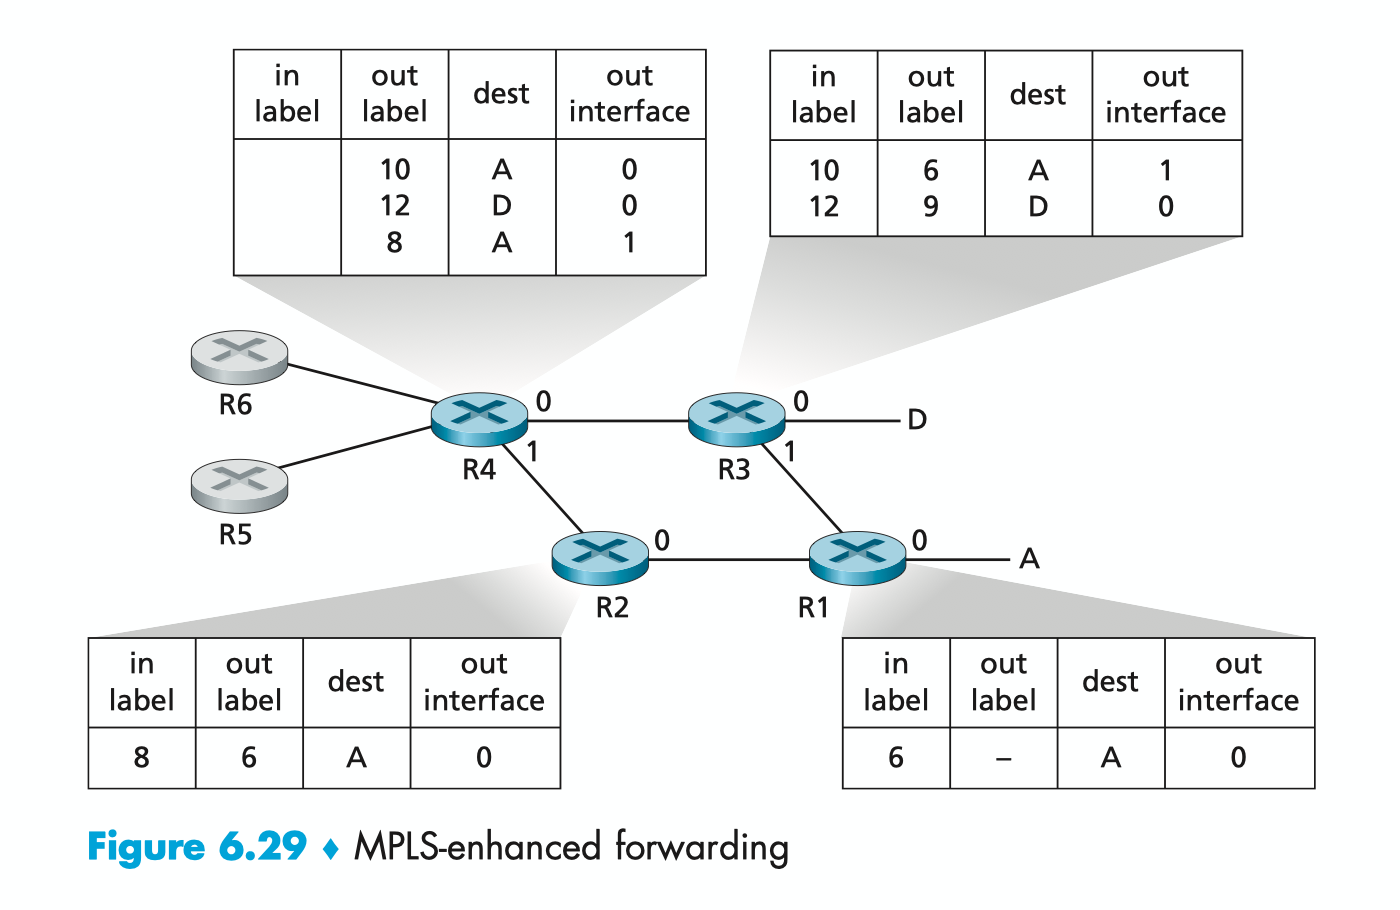
\includegraphics[width=0.65\textwidth]{Fig6.29.png}
    \end{figure}
    \item P33. Consider the hierarchical network in Figure 6.30 and suppose that the data center needs to support e-mail and video distribution among other applications. Suppose four racks of servers are reserved for e-mail and four racks are reserved for video. For each of the applications, all four racks must lie below a single tier-2 switch since the tier-2 to tier-1 links do not have sufficient bandwidth to support the intra-application traffic. For the e-mail application, suppose that for 99.9 percent of the time only three racks are used, and that the video application has identical usage patterns.
    \begin{figure}[h!]
        \centering
        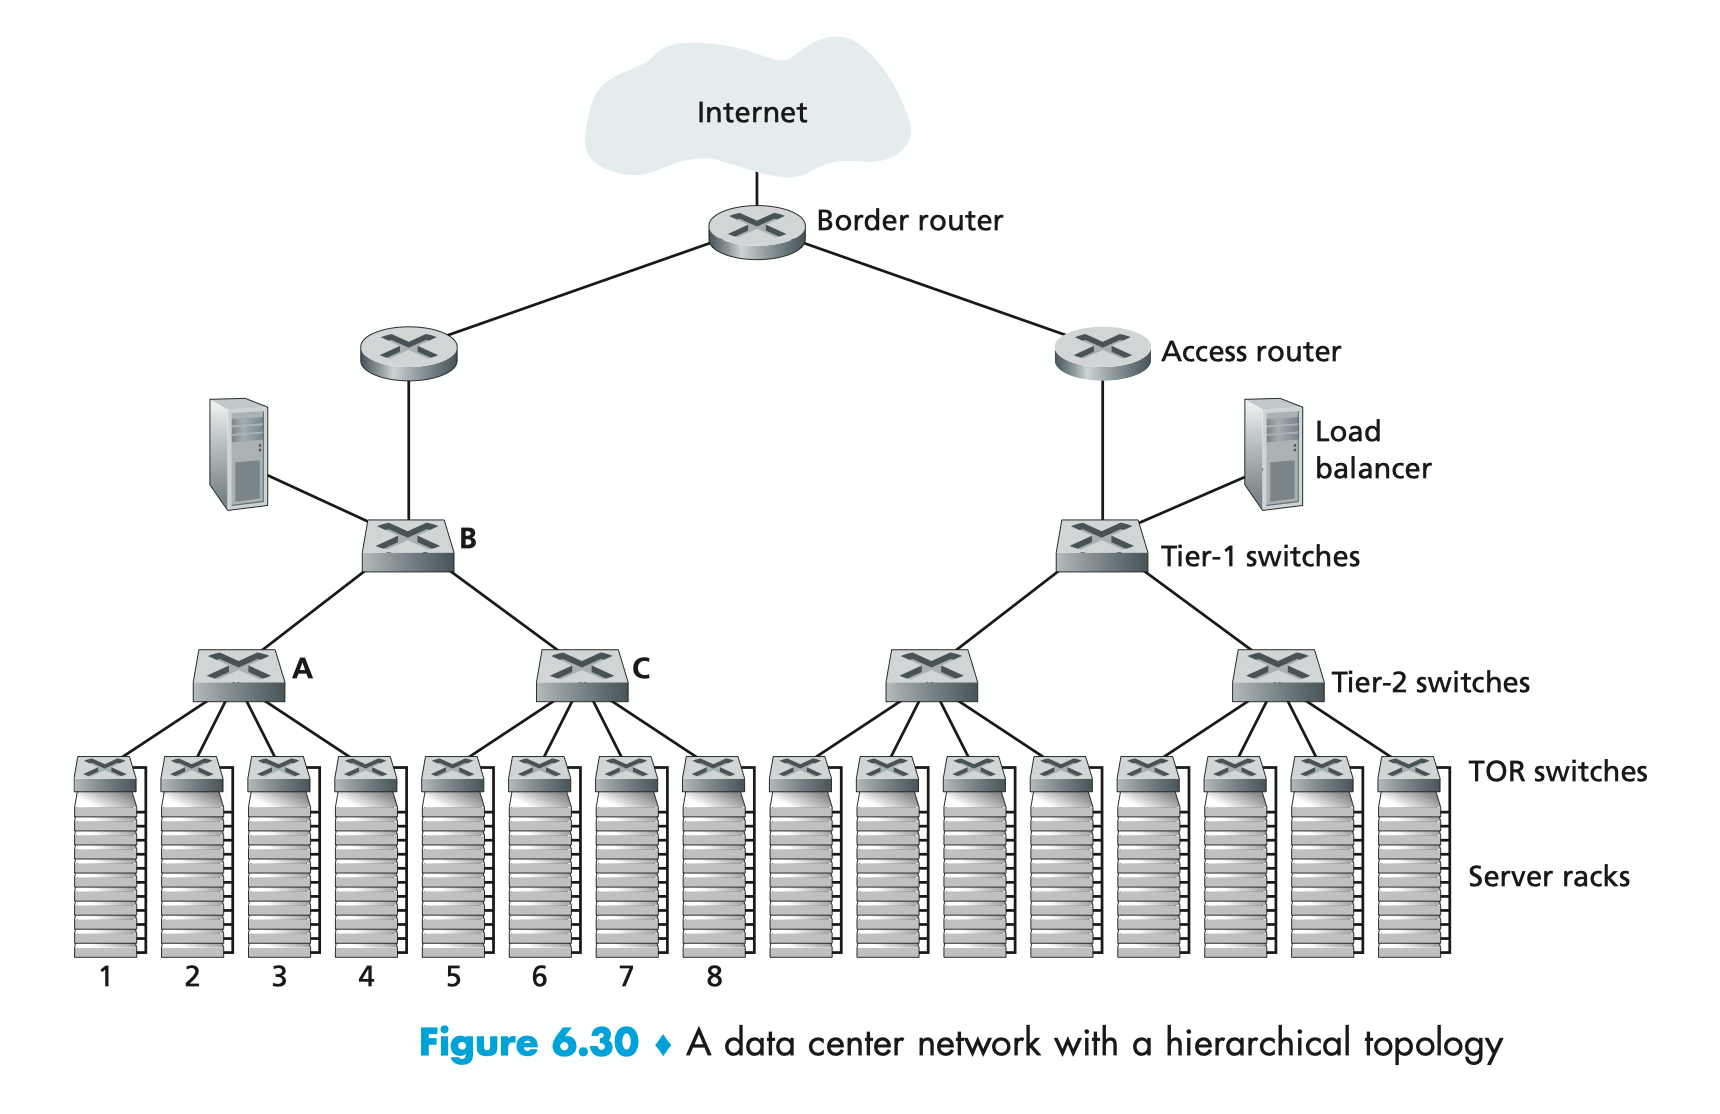
\includegraphics[width=0.73\textwidth]{Fig6.30.png}
    \end{figure}\newpage
    \begin{enumerate}
        \item For what fraction of time does the e-mail application need to use a fourth rack? How about for the video application?\\[1em]
        The problem states that for the e-mail application, 99.9 percent of the time only three racks are used; therefore, 0.1 percent of the time, a fourth rack will be needed. The video application has identical usage patterns.
        \item Assuming e-mail usage and video usage are independent, for what fraction of time do (equivalently, what is the probability that) both applications need their fourth rack?\\[1em]
        The probability that both applications need their fourth rack is \(0.1\% \cdot 0.1\% = 0.000001\).
        \item Suppose that it is acceptable for an application to have a shortage of servers for 0.001 percent of time or less (causing rare periods of performance degradation for users). Discuss how the topology in Figure 6.31 can be used so that only seven racks are collectively assigned to the two applications (assuming that the topology can support all the traffic).
        \begin{figure}[h!]
            \centering
            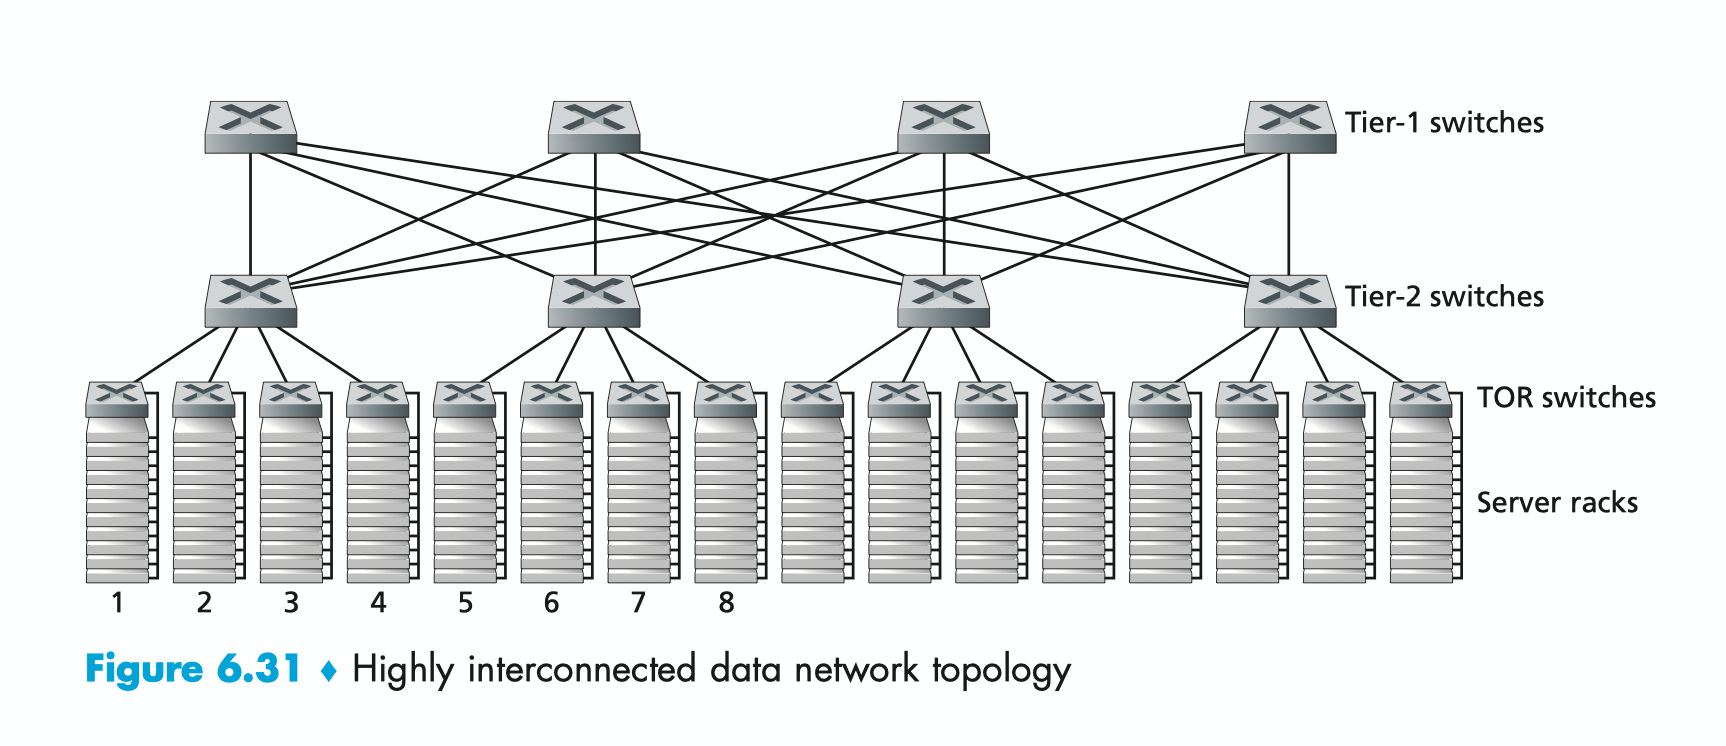
\includegraphics[width=0.75\textwidth]{Fig6.31.png}
        \end{figure}\\[1em]
        In part (b) we found that the probability of both the e-mail application and the video application both needing a fourth rack at the same time is 0.000001 or 0.0001\%. With this topology, the video application and the e-mail application can each have their own dedicated three racks, sharing a seventh rack between them for overflow. So long as they both do not need the overflow rack at the same time (0.0001\%) there should not be any issues; this is well below the stated acceptable shortage of 0.001\%.
    \end{enumerate}
\end{enumerate}
\end{document}